\chapter{Results}\label{results}

This chapter reports the four models on the 524 held-out matches (section \ref{res:models}), the features they rely on (section \ref{res:importance}), what the model says about teams and players (section \ref{res:teams}), and whether one model can serve different leagues (section \ref{res:leagues}).

\section{Model Validation}\label{res:models}

Table \ref{tab:models} shows the results of the four tuned models on the held-out test matches: 12,009 open-play shots and 1,253 goals. StatsBomb's own xG for the same shots is included as a reference point.

\begin{table}[!h]
\centering
\small
\begin{tabular}{|l|c|c|c|c|c|c|}
\hline
\textbf{Model} & \textbf{CV log loss} & \textbf{Log loss} & \textbf{Brier} & \textbf{AUC} & \textbf{ECE} & \textbf{xG ÷ goals} \\
\hline
Logistic Regression & 0.2655 & 0.2699 & 0.0776 & 0.804 & 0.0047 & 1.00 \\
XGBoost & 0.2640 & 0.2686 & 0.0771 & 0.806 & 0.0058 & 0.99 \\
LightGBM & 0.2642 & 0.2696 & 0.0774 & 0.804 & 0.0065 & 0.99 \\
\textbf{CatBoost} & \textbf{0.2637} & 0.2687 & 0.0772 & 0.806 & 0.0048 & 0.99 \\
\hline
StatsBomb xG & -- & 0.2647 & 0.0759 & 0.813 & 0.0101 & 0.94 \\
\hline
\end{tabular}
\caption{Results on 524 held-out matches. CV log loss is the cross-validated log loss on the training matches, used to choose the final model.}
\label{tab:models}
\end{table}

\textbf{CatBoost} had the best cross-validated log loss and was chosen as the final model, before the test set was used. Its tuned settings were a tree depth of 7, 302 trees, a learning rate of 0.025 and an L2 regularisation of 4.56. The tuned Logistic Regression used $C = 0.144$.

\subsection{The Choice of Algorithm barely Matters}

The four models are almost tied. On the test matches, their log loss differs by at most 0.0013 and their AUC by 0.002, and their ROC curves lie on top of each other (figure \ref{fig:roc}). To check whether the differences are real, the test matches were resampled 2,000 times (a match bootstrap, so that shots from one match stay together). CatBoost's log loss was 0.0012 lower than Logistic Regression's, but the 95\% interval ($-0.0029$ to $+0.0004$) includes zero, so the simplest model cannot be said to be worse. CatBoost was indistinguishable from XGBoost, and slightly but clearly better than LightGBM (by 0.0010; interval $-0.0018$ to $-0.0001$).

\begin{figure}[!h]
    \centering
    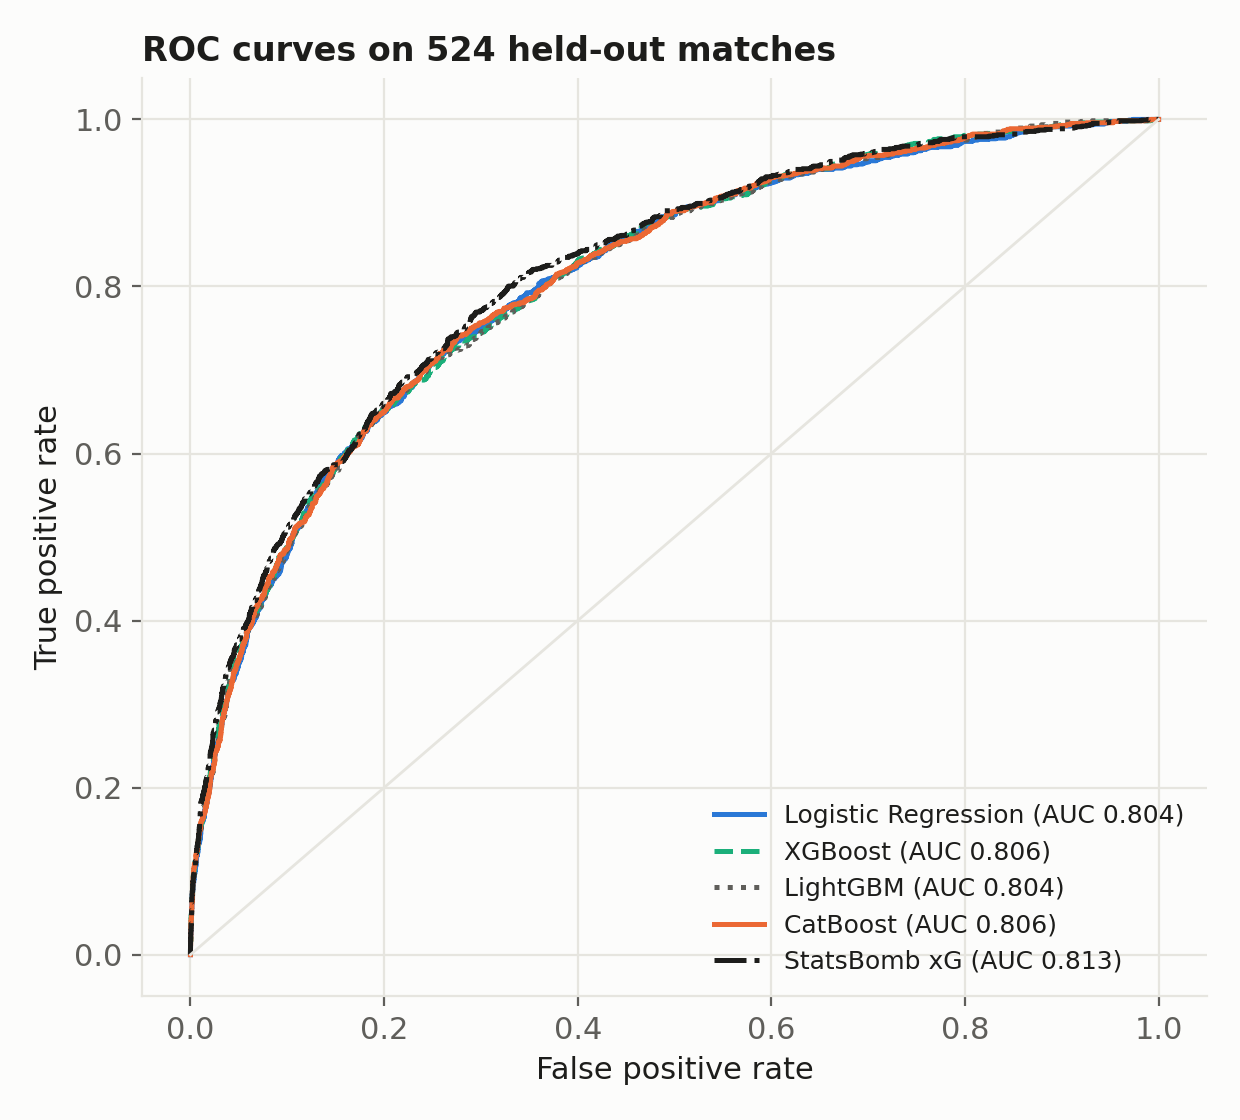
\includegraphics[width=0.65\textwidth]{images/roc.png}
    \caption{ROC Curves on the Held-out Matches}
    \label{fig:roc}
\end{figure}

\subsection{Predictions match Reality}

All four models are well calibrated. Their calibration error is about half a percentage point, and they predict between 98.7\% and 99.6\% of the goals actually scored in the test matches; the 95\% intervals, roughly $\pm$4.5\%, all include 100\%. Figure \ref{fig:calibration} shows the calibration of CatBoost: in each group of shots, from the least to the most promising, the mean xG is close to the share of goals.

\begin{figure}[!h]
    \centering
    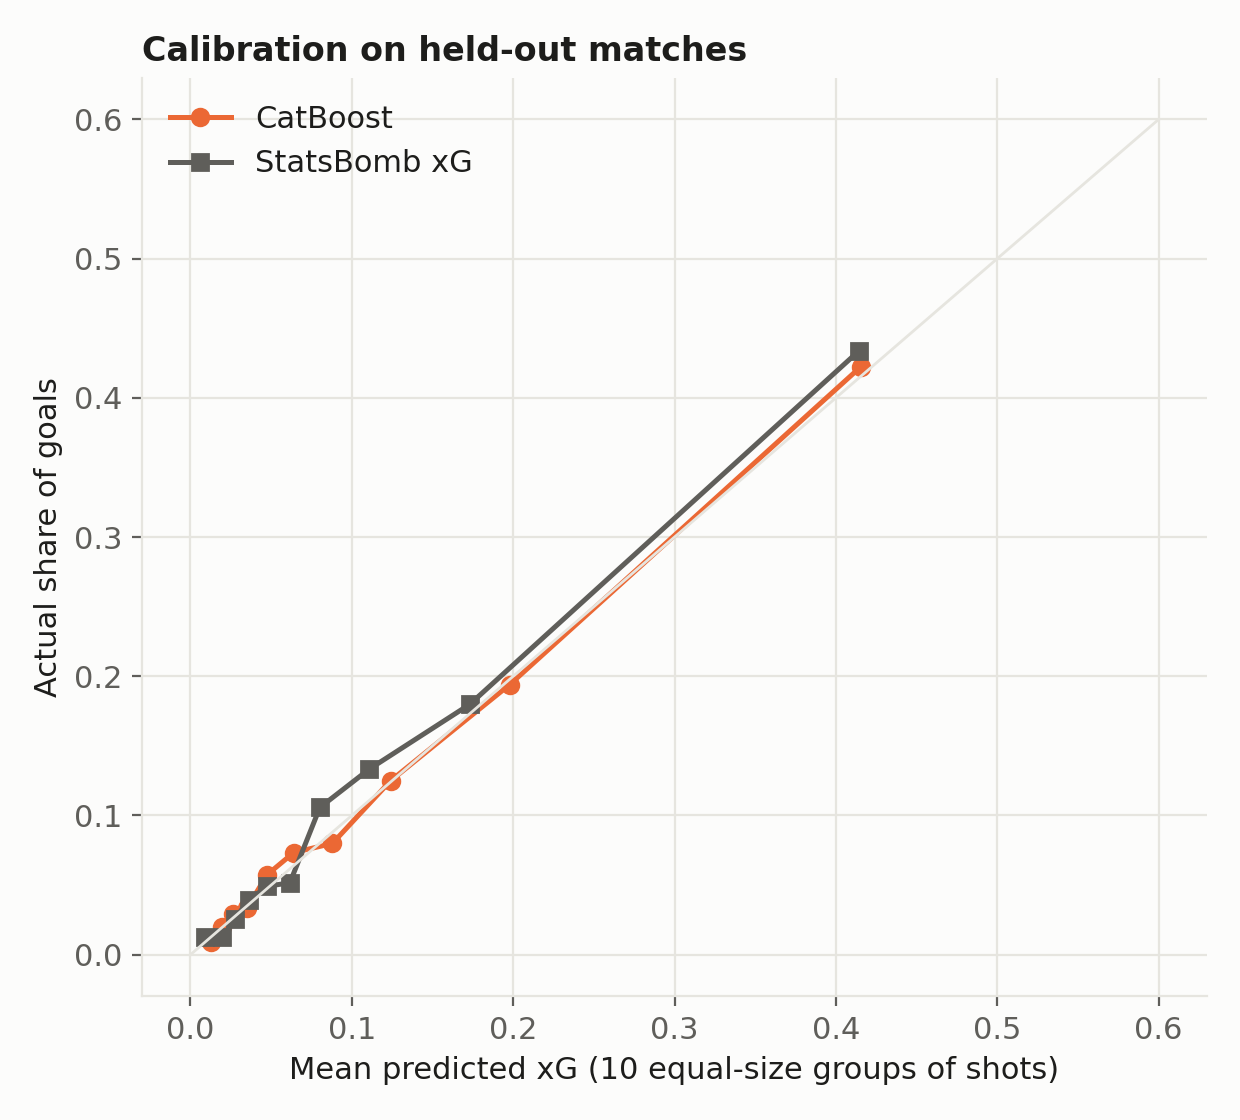
\includegraphics[width=0.65\textwidth]{images/calibration.png}
    \caption{Calibration on the Held-out Matches}
    \label{fig:calibration}
\end{figure}

\subsection{Comparison with StatsBomb xG}

StatsBomb's xG scores better on log loss (by 0.0039; interval 0.0018 to 0.0061) and AUC (0.813 against 0.806). It is a reference point rather than a fair competitor: StatsBomb trains its model on far more data and on information beyond these 13 features, very likely including these same matches. StatsBomb's xG is less well calibrated on these matches, however: it predicts 6\% fewer goals than were scored (0.94; interval 0.90 to 0.98).

\subsection{Comparison with the Original Edition}

The original edition reported AUC scores between 0.80 and 0.82, against 0.84 for StatsBomb. Those scores were measured on Barcelona's matches, with shots from the same match on both sides of a random split. The scores here (0.804--0.806) are measured on unseen matches from many competitions. They are a harder and fairer test, not a drop in quality.

Every shot also has an out-of-fold xG from a model that never saw its match (section \ref{test}). Across all 61,003 shots these have a log loss of 0.2645, an AUC of 0.809 and a calibration error of 0.003, and they predict 99.7\% of the goals scored.

\newpage

\section{Feature Importance}\label{res:importance}

To see which features each model relies on, every feature was shuffled in turn on the test matches, which breaks its link with the outcome, and the increase in log loss was measured (permutation importance, averaged over 5 shuffles). Figure \ref{fig:importance} shows the result for Logistic Regression and CatBoost.

\begin{figure}[!h]
    \centering
    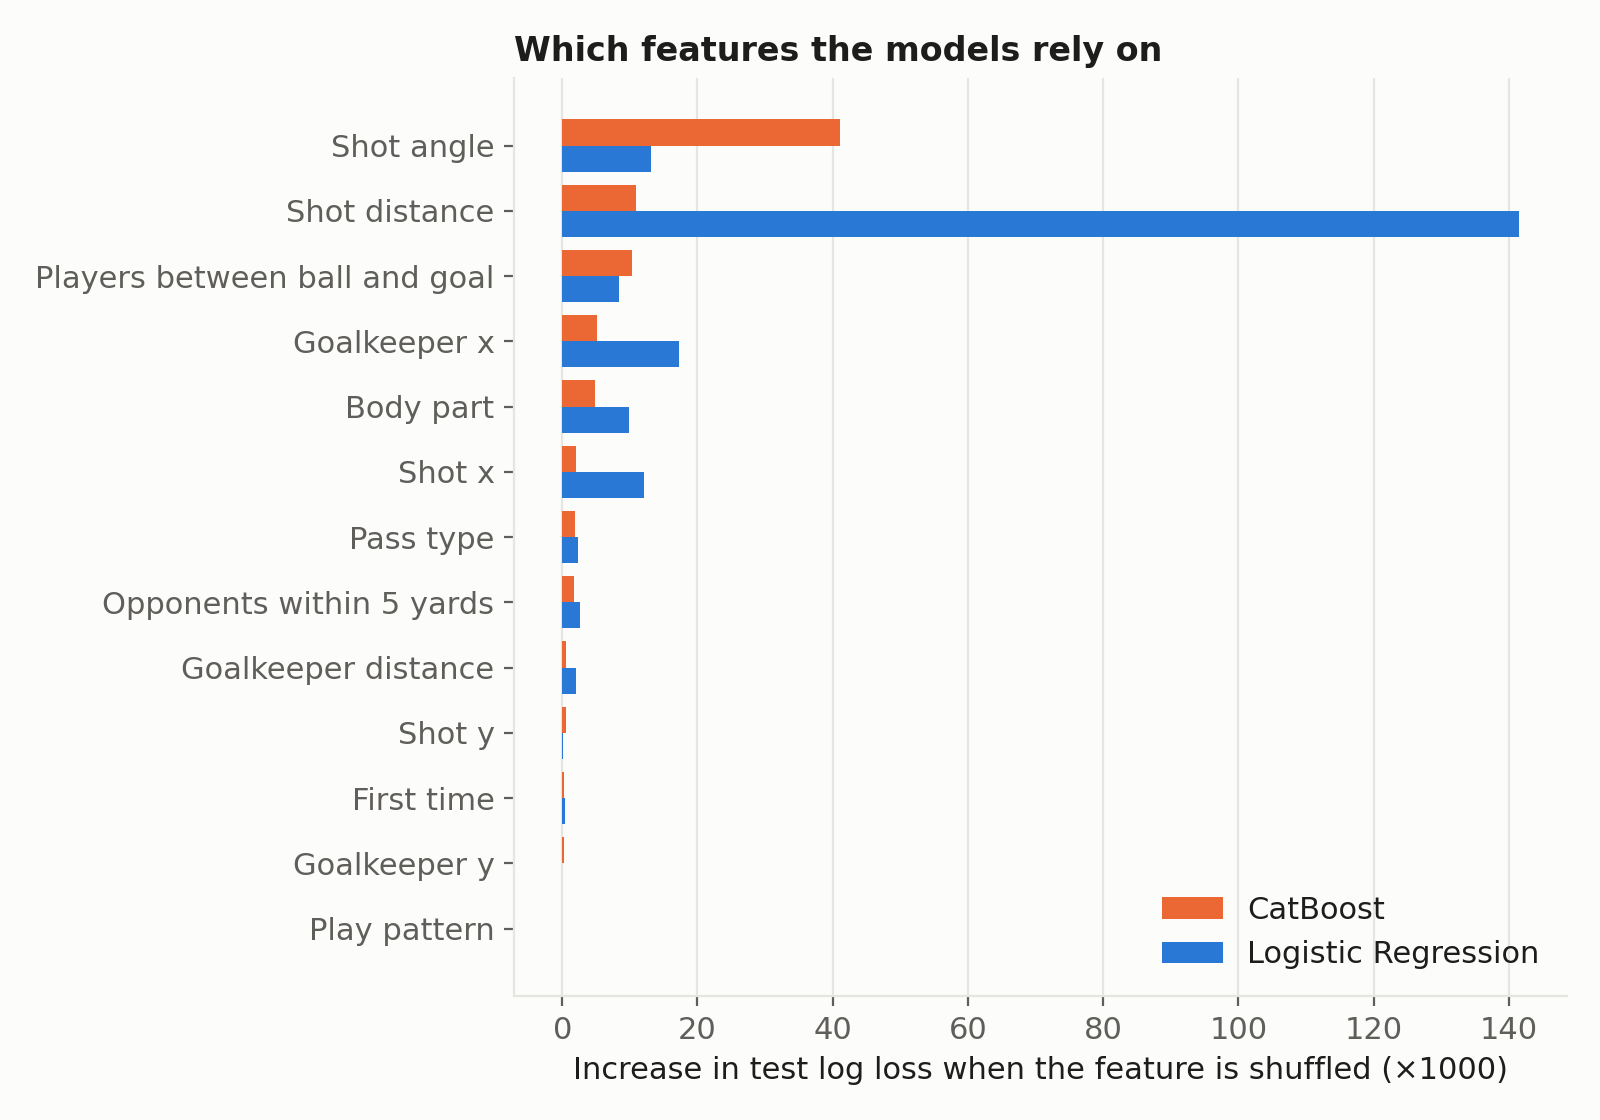
\includegraphics[width=0.9\textwidth]{images/importance.png}
    \caption{Permutation Importance on the Held-out Matches}
    \label{fig:importance}
\end{figure}

Both models rely on the geometry of the shot, but they divide the credit differently:
\begin{itemize}
    \item \textbf{Logistic Regression} relies above all on shot distance (an increase of 0.142 in log loss when it is shuffled), followed by the goalkeeper's x coordinate, shot angle, the shot's x coordinate, body part and the players between the ball and goal.
    \item \textbf{CatBoost} relies most on shot angle (0.041), followed by shot distance and the players between the ball and goal (0.011 and 0.010), then the goalkeeper's x coordinate and body part (0.005 each).
\end{itemize}

The difference is a consequence of how the two models work, not a disagreement about football. Shot distance, shot angle and the shot's x coordinate carry much of the same information. A linear model needs distance to describe how the chance falls away from goal, while the trees of CatBoost can take the same information from the angle. When features overlap, permutation importance shares the credit between them in a way that depends on the model, so the ranking within this group should not be read too literally.

The features that matter little are clearer. Pressure, pass type, goalkeeper distance and the shot's y coordinate add a little. First time and the goalkeeper's y coordinate add almost nothing once the rest is known, and play pattern adds nothing at all in either model. As discussed in the exploratory analysis, grouping the play patterns into Regular and Non Regular Play hides the one pattern that stands out, the counter attack.

\newpage

\section{Teams and Players}\label{res:teams}

The tables in this section use the out-of-fold xG, so each shot's xG comes from a model that never saw its match. They count open-play shots and goals only, the shots the model covers; penalties, direct free kicks and own goals are not included, so ``goals'' here is lower than official totals.

\subsection{League Tables 2015/16}

StatsBomb's open data contains the full 2015/16 seasons of the Premier League, La Liga and Serie A, and all but 3 matches of Ligue 1. The points and positions calculated from the match results match the official final tables exactly for the first three leagues. Table \ref{tab:spearman} shows how well each team's xG difference (xG for minus xG against) tracks its points.

\begin{table}[!h]
\centering
\begin{tabular}{|l|c|c|c|}
\hline
\textbf{League} & \textbf{Matches} & \textbf{xG diff. vs points} & \textbf{Goal diff. vs points} \\
\hline
Premier League & 380 & 0.85 & 0.93 \\
La Liga & 380 & 0.73 & 0.85 \\
Serie A & 380 & 0.83 & 0.95 \\
Ligue 1 & 377 & 0.61 & 0.65 \\
\hline
\end{tabular}
\caption{Rank correlation (Spearman) of open-play xG difference and open-play goal difference with points, 2015/16}
\label{tab:spearman}
\end{table}

xG difference tracks the table well, though less closely than actual goal difference. That is expected, since points are decided by actual goals. xG measures the quality of the chances a team created and allowed, and the gap between the two shows which teams did better or worse than their chances.

The 2015/16 Premier League is a famous example (figure \ref{fig:pl} and table \ref{tab:pl}). Leicester City won the league with 81 points while ranking only 6th on open-play xG difference; among other things, they conceded 32 open-play goals from chances worth 44.6 xG. Arsenal had the best xG difference in the league (+34.1) and finished second, 10 points behind. Aston Villa were last on both measures.

\begin{figure}[!h]
    \centering
    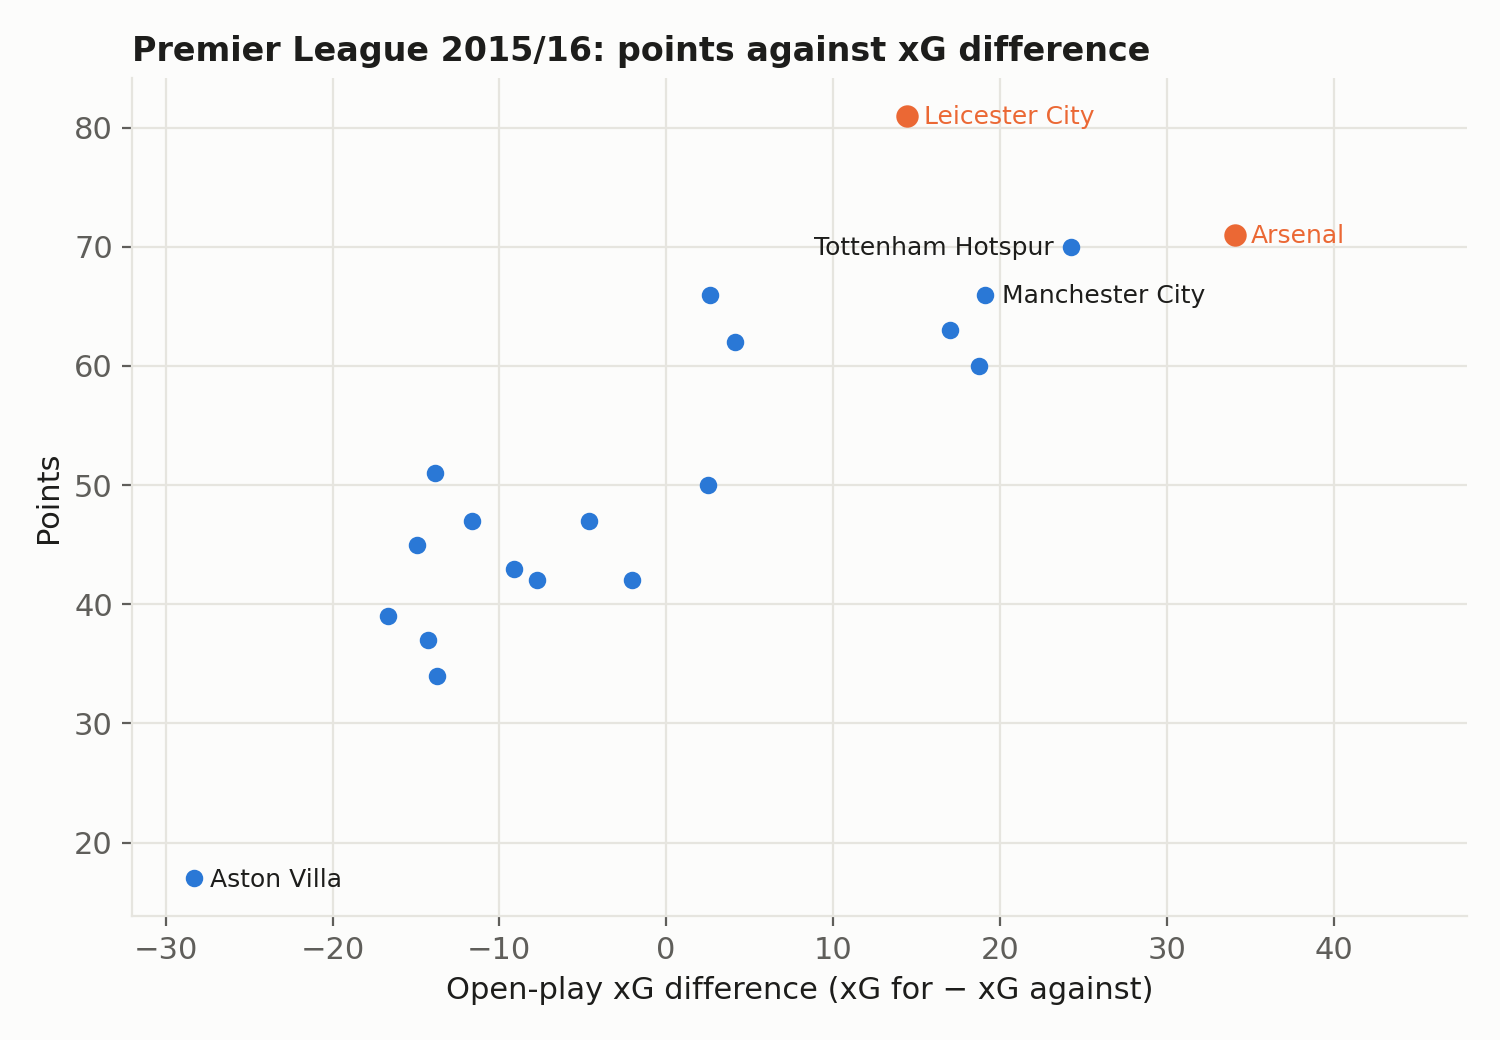
\includegraphics[width=0.8\textwidth]{images/pl_2015_16.png}
    \caption{Premier League 2015/16: Points against Open-play xG Difference}
    \label{fig:pl}
\end{figure}

\begin{table}[!h]
\centering
\small
\begin{tabular}{|c|l|c|c|c|c|c|c|c|}
\hline
\textbf{Pos} & \textbf{Team} & \textbf{Pts} & \textbf{GF} & \textbf{xGF} & \textbf{GA} & \textbf{xGA} & \textbf{xG diff} & \textbf{xG rank} \\
\hline
1 & Leicester City & 81 & 56 & 59.0 & 32 & 44.6 & 14.4 & 6 \\
2 & Arsenal & 71 & 61 & 68.8 & 30 & 34.8 & 34.1 & 1 \\
3 & Tottenham Hotspur & 70 & 60 & 59.7 & 31 & 35.4 & 24.2 & 2 \\
4 & Manchester City & 66 & 62 & 58.6 & 39 & 39.4 & 19.1 & 3 \\
5 & Manchester United & 66 & 42 & 40.7 & 29 & 38.1 & 2.6 & 8 \\
6 & Southampton & 63 & 53 & 54.7 & 37 & 37.6 & 17.0 & 5 \\
7 & West Ham United & 62 & 57 & 53.4 & 40 & 49.2 & 4.2 & 7 \\
8 & Liverpool & 60 & 57 & 56.8 & 48 & 38.0 & 18.8 & 4 \\
9 & Stoke City & 51 & 35 & 37.6 & 48 & 51.5 & -13.8 & 16 \\
10 & Chelsea & 50 & 47 & 51.4 & 47 & 48.9 & 2.5 & 9 \\
11 & Everton & 47 & 50 & 50.0 & 49 & 54.6 & -4.6 & 11 \\
12 & Swansea City & 47 & 32 & 39.1 & 40 & 50.7 & -11.6 & 14 \\
13 & Watford & 45 & 30 & 38.3 & 42 & 53.2 & -15.0 & 18 \\
14 & West Bromwich Albion & 43 & 29 & 36.0 & 37 & 45.2 & -9.1 & 13 \\
15 & Crystal Palace & 42 & 34 & 40.9 & 39 & 48.6 & -7.7 & 12 \\
16 & AFC Bournemouth & 42 & 40 & 41.6 & 60 & 43.6 & -2.1 & 10 \\
17 & Sunderland & 39 & 35 & 38.8 & 55 & 55.5 & -16.7 & 19 \\
18 & Newcastle United & 37 & 39 & 39.5 & 57 & 53.8 & -14.3 & 17 \\
19 & Norwich City & 34 & 36 & 40.0 & 58 & 53.8 & -13.7 & 15 \\
20 & Aston Villa & 17 & 24 & 29.4 & 61 & 57.7 & -28.3 & 20 \\
\hline
\end{tabular}
\caption{Premier League 2015/16 with open-play goals (GF, GA) and xG (xGF, xGA)}
\label{tab:pl}
\end{table}

In La Liga, the top three (Barcelona, Real Madrid and Atlético Madrid) were also the top three on xG difference, while Villarreal finished 4th with only the 11th best xG difference. In Serie A, Napoli had a slightly better xG difference than the champions Juventus. The full tables for all four leagues are in the project repository (\texttt{docs/TABLES.md}).

\newpage

\subsection{Finishing: Goals against xG}

xG describes how good a player's chances were; comparing it with the goals the player actually scored shows how well the chances were taken. Because luck plays a large part, the gap is also expressed as a $z$ score: the difference between goals and xG divided by how much that difference would vary by chance for an average finisher taking the same shots,
\begin{equation}
z = \frac{\text{goals} - \sum_i p_i}{\sqrt{\sum_i p_i(1 - p_i)}}
\end{equation}
where $p_i$ is the xG of each shot. Roughly, a $|z|$ above 2 is unlikely to be luck alone.

\begin{figure}[!h]
    \centering
    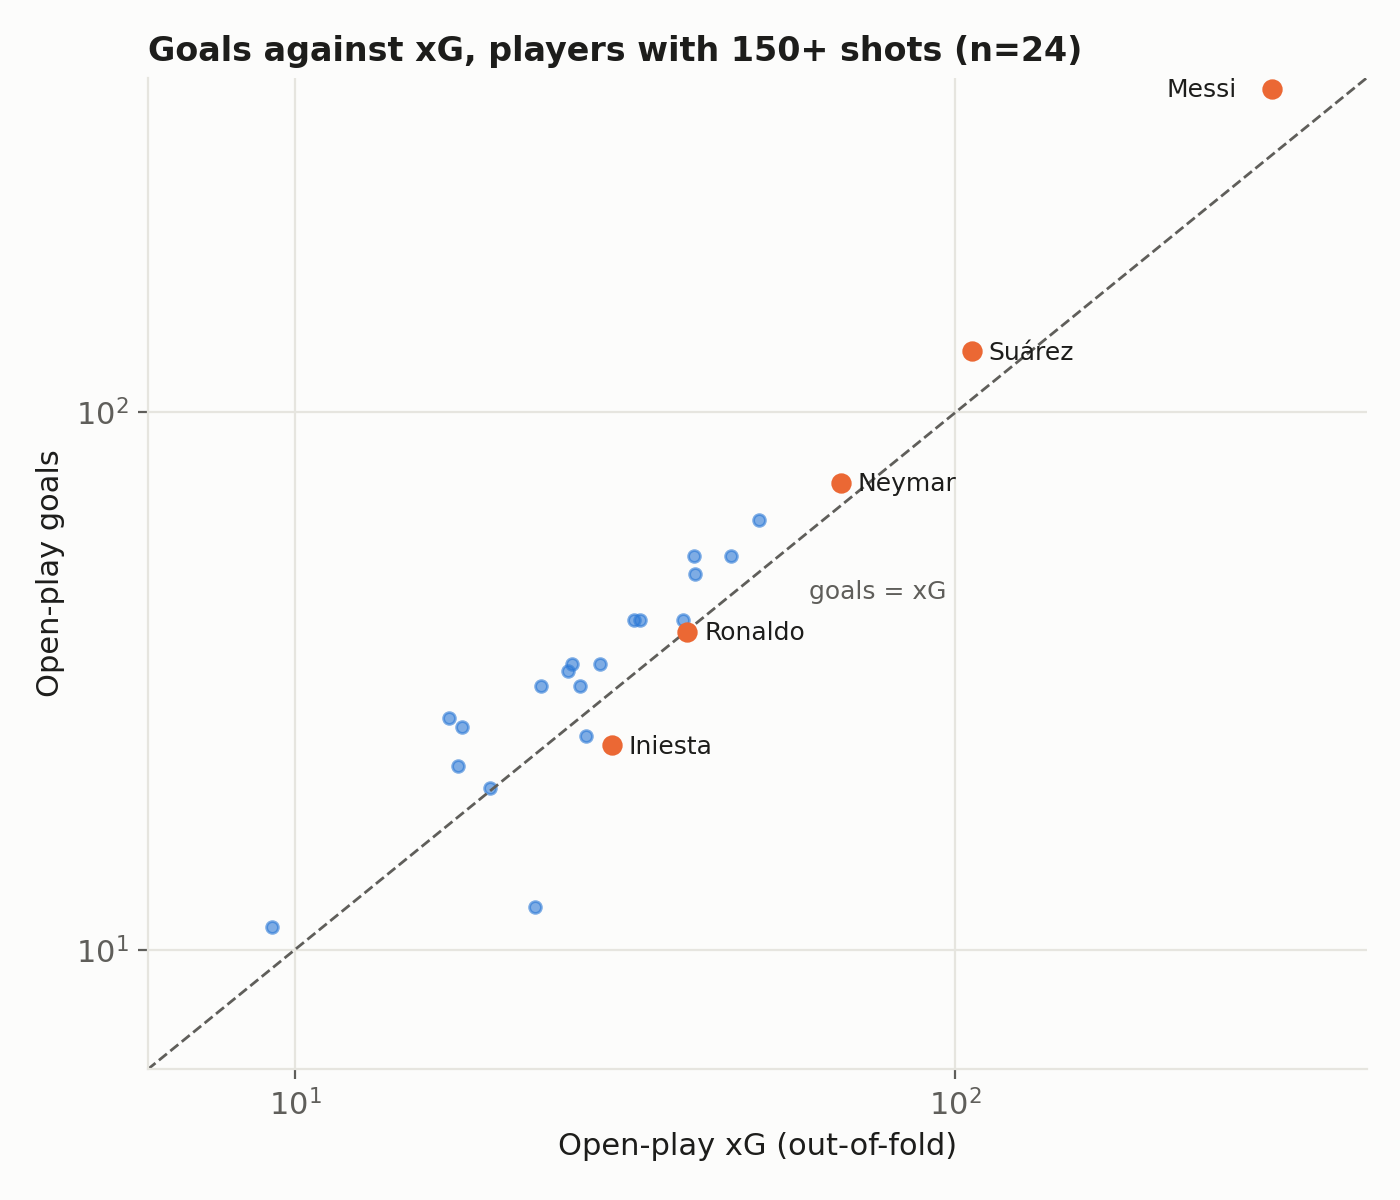
\includegraphics[width=0.75\textwidth]{images/players.png}
    \caption{Open-play Goals against xG, Players with at least 150 Shots (log scales)}
    \label{fig:players}
\end{figure}

\begin{table}[!h]
\centering
\begin{tabular}{|l|c|c|c|c|c|}
\hline
\textbf{Player} & \textbf{Shots} & \textbf{Goals} & \textbf{xG} & \textbf{Goals $-$ xG} & \textbf{$z$} \\
\hline
Lionel Messi & 2,107 & 400 & 301.2 & +98.8 & +6.8 \\
Luis Suárez & 601 & 130 & 106.0 & +24.0 & +2.9 \\
Kylian Mbappé & 288 & 54 & 40.2 & +13.8 & +2.6 \\
Samuel Eto'o & 295 & 63 & 50.4 & +12.6 & +2.2 \\
Neymar & 407 & 74 & 67.2 & +6.8 & +1.0 \\
Cristiano Ronaldo & 320 & 39 & 39.3 & $-$0.3 & $-$0.1 \\
Andrés Iniesta & 367 & 24 & 30.2 & $-$6.2 & $-$1.3 \\
Martin Braithwaite & 156 & 12 & 23.1 & $-$11.1 & $-$2.8 \\
\hline
\end{tabular}
\caption{Open-play finishing of selected players with at least 150 shots in the open data}
\label{tab:finishing}
\end{table}

\textbf{Lionel Messi} is the outstanding finisher in the data (figure \ref{fig:players} and table \ref{tab:finishing}). From 2,107 open-play shots he scored 400 goals against 301.2 xG, almost 99 goals more than an average finisher would have scored from the same chances, and a $z$ score of +6.8 rules out luck. Luis Suárez (+24.0, $z$ = +2.9) and Kylian Mbappé (+13.8, $z$ = +2.6) also clearly beat their xG. Neymar scored slightly more than his xG, within what luck could explain.

\textbf{Andrés Iniesta} scored 24 goals from 367 shots, 6.2 fewer than his xG ($z$ = $-$1.3, within the range of luck). The bigger reason for his low tally is the chances themselves: his average shot was worth 0.082 xG, against 0.103 for all shots in the data. Iniesta mostly shot from positions where goals are unlikely, which fits a playmaker who created chances for others.

The coverage of the open data should be kept in mind: Barcelona's players appear in every Barcelona La Liga match from 2004/05 to 2020/21, while most other players appear only in the competitions and seasons the open data covers. Cristiano Ronaldo's 320 shots, for example, cover only a small part of his career.

\subsection{Barcelona}

The same finishing quality shows at team level. Barcelona scored more open-play goals than their xG in 15 of the 17 La Liga seasons in the data (figure \ref{fig:barca}), with the peak in 2012/13: 85 goals from chances worth 51.6 xG. On Barcelona's shots in the test matches, the model predicts 15\% fewer goals than they scored, while it predicts the goals of all other teams within 1\%.

\begin{figure}[!h]
    \centering
    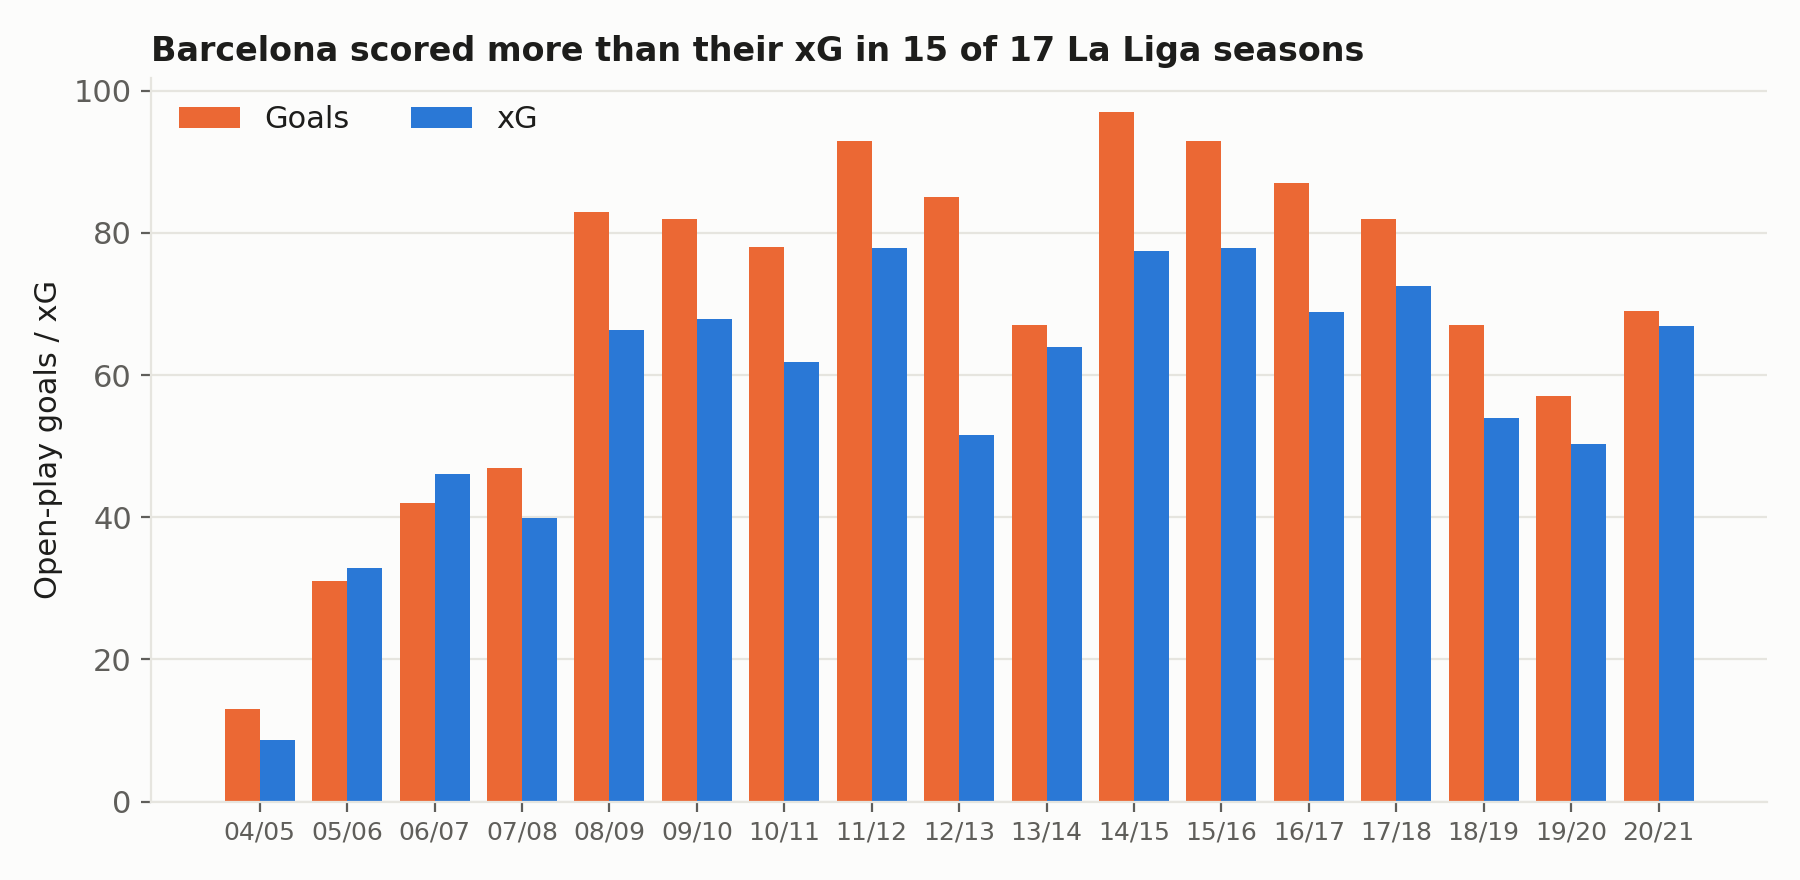
\includegraphics[width=0.9\textwidth]{images/barcelona_seasons.png}
    \caption{Barcelona in La Liga: Open-play Goals and xG by Season}
    \label{fig:barca}
\end{figure}

\newpage

\section{One Model for Different Leagues?}\label{res:leagues}

Each league has its own style of play, which raises the question whether a model trained on several leagues is biased for each of them. This was tested on the four complete 2015/16 seasons: 35,645 open-play shots from 1,517 matches. The matches of each league were split into 5 folds, and every held-out fold was predicted by models trained in four ways:
\begin{itemize}
    \item \textbf{Pooled}: trained on all four leagues
    \item \textbf{Own league only}: a separate model for each league
    \item \textbf{Other three only}: trained without the league being predicted, a direct test of whether a model transfers between styles
    \item \textbf{Pooled with a league feature}: told which league each shot is from, so it can learn an adjustment for each league
\end{itemize}

CatBoost and Logistic Regression were used, with the settings tuned in section \ref{res:models}. The 95\% intervals come from resampling whole matches.

\begin{table}[!h]
\centering
\resizebox{\textwidth}{!}{%
\begin{tabular}{|l|c|c|c|c|c|}
\hline
\textbf{League} & \textbf{Pooled} & \textbf{Own league} & \textbf{Other three} & \textbf{League feature} & \textbf{StatsBomb} \\
\hline
Premier League & 1.03 (0.96--1.10) & 0.98 (0.92--1.05) & 1.04 (0.97--1.11) & 1.01 (0.94--1.08) & 1.00 (0.93--1.07) \\
La Liga & 0.99 (0.93--1.04) & 0.98 (0.93--1.04) & 0.99 (0.93--1.04) & 0.99 (0.94--1.05) & 0.97 (0.91--1.02) \\
Serie A & 0.99 (0.93--1.05) & 0.98 (0.92--1.04) & 0.99 (0.93--1.05) & 0.99 (0.93--1.05) & 0.98 (0.93--1.04) \\
Ligue 1 & 0.98 (0.92--1.04) & 0.98 (0.92--1.05) & 0.97 (0.91--1.04) & 0.98 (0.92--1.05) & 0.96 (0.90--1.02) \\
\hline
\end{tabular}}
\caption{Predicted ÷ actual goals per league, CatBoost, with 95\% intervals}
\label{tab:leaguecal}
\end{table}

\begin{figure}[!h]
    \centering
    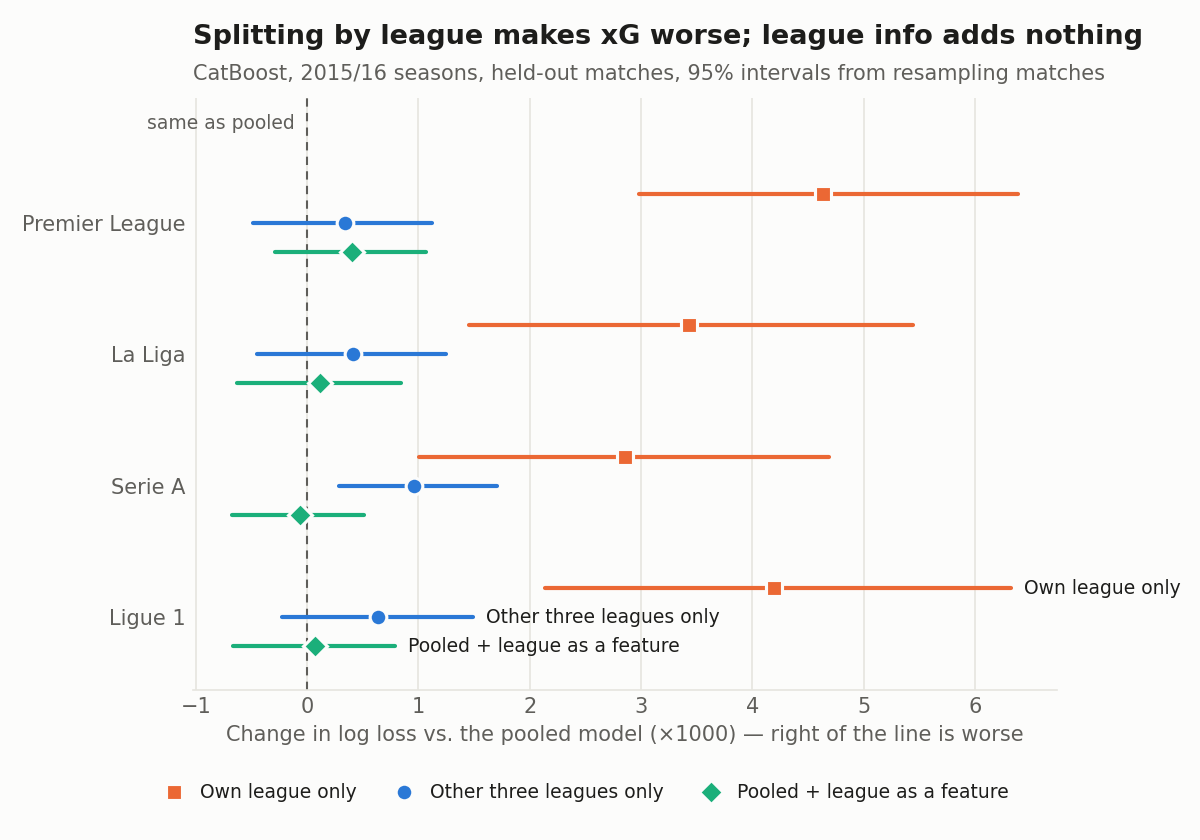
\includegraphics[width=0.9\textwidth]{images/leagues.png}
    \caption{Change in Log Loss compared with the Pooled Model, per League}
    \label{fig:leagues}
\end{figure}

The results are clear:
\begin{enumerate}
    \item \textbf{Mixing the four leagues does not bias the model.} The pooled model is calibrated in each league (between 0.98 and 1.03 of the actual goals), and every interval includes 1.00 (table \ref{tab:leaguecal}).
    \item \textbf{A model transfers to a league it has not seen.} The model trained on the other three leagues is calibrated in all four, and its log loss is only 0.0003--0.0010 higher than the pooled model's.
    \item \textbf{Separate models per league are worse.} With CatBoost, the own-league models have a clearly higher log loss than the pooled model in all four leagues, by 0.0029 to 0.0046 (figure \ref{fig:leagues}). That is more than the whole gap between the four algorithms in section \ref{res:models}: having fewer shots to learn from costs more than specialising gains. The simpler Logistic Regression loses less from splitting, but never gains.
    \item \textbf{Telling the model the league adds nothing.} The pooled model with a league feature is indistinguishable from the pooled model in every league, for both algorithms.
\end{enumerate}

A league of a different standard is another matter. The model trained on the four European leagues predicts 12\% fewer goals than were scored in the Indian Super League 2021/22 (0.88; interval 0.80 to 0.98), and StatsBomb's own model shows the same gap (0.89). The difference there is plausibly one of finishing and goalkeeping quality rather than style, and xG for such a league should be recalibrated or used with care.
